\section{Regret matching: the ten-line rule the whole field runs on}\label{sec:rm}

\mkey{regret matching}Strip poker away entirely and start with rock--paper--scissors. The engine underneath every solver in this survey is a 2000 learning rule by Hart and Mas-Colell called \keyterm{regret matching}\mdef{regret matching}{play each action with probability proportional to its accumulated positive regret}~\cite{hart2000}. After each round, ask for every action: \emph{how much better would I have done had I always played that instead?} Add that gap --- the \keyterm{regret}\mdef{regret}{hindsight gap: (what action $a$ would have paid) $-$ (what I actually got)} --- to a running ledger per action. Next round, play actions in proportion to their positive ledger entries.

\begin{lstlisting}
ledger = {a: 0 for a in ACTIONS}            # cumulative regret per action

def strategy():                              # regret matching
    pos = {a: max(r, 0) for a, r in ledger.items()}
    Z = sum(pos.values())
    return {a: p/Z for a, p in pos.items()} if Z > 0 else uniform()

def update(my_action, their_action):
    for a in ACTIONS:                        # the what-if ledger update
        ledger[a] += payoff(a, their_action) - payoff(my_action, their_action)
\end{lstlisting}

\mnote{\textbf{Rail trace} --- round 1, I throw Rock, they throw Paper (payoff $-1$):\\
what-ifs: Paper $\to 0$, Scissors $\to +1$.\\
ledger: P ${+}{=}\,1$, S ${+}{=}\,2$, R ${+}{=}\,0$\\
next play: P $\tfrac13$, S $\tfrac23$, R $0$.\\
Round 2, I throw Scissors, they hold Paper ($+1$): ledger $\to$ R $-2$, P $0$, S $+2$ --- all-in on Scissors, and the chase begins.}Notice what is \emph{absent}: no learning rate, no optimizer, no gradient --- accumulate and normalize. Hart and Mas-Colell proved this rule is a \keyterm{no-regret learner}\mdef{no-regret learner}{average regret per round provably shrinks toward zero as play continues}: its average regret vanishes over time no matter what the opponent does. That property, not any poker insight, is the load-bearing theorem of computer poker.

Because when \emph{both} players run regret-matching against each other, two things happen at once, and Figure~\ref{fig:rps} shows them with a real simulation. The \emph{current} strategies chase each other forever --- I over-throw Scissors, you learn Rock, I learn Paper, and the ledgers keep circling. But a folk theorem of game theory converts vanishing regret into equilibrium: \hlight{in a two-player zero-sum game, if both players' average regret is $\varepsilon$, the pair of \emph{time-averaged} strategies is a $2\varepsilon$-Nash equilibrium.} The orbit never stops; the \emph{center of the orbit} is the answer. In the figure the running average settles onto exactly $\tfrac13,\tfrac13,\tfrac13$ --- the unexploitable RPS strategy --- while the current strategy never settles at all.

\begin{figure}[t]
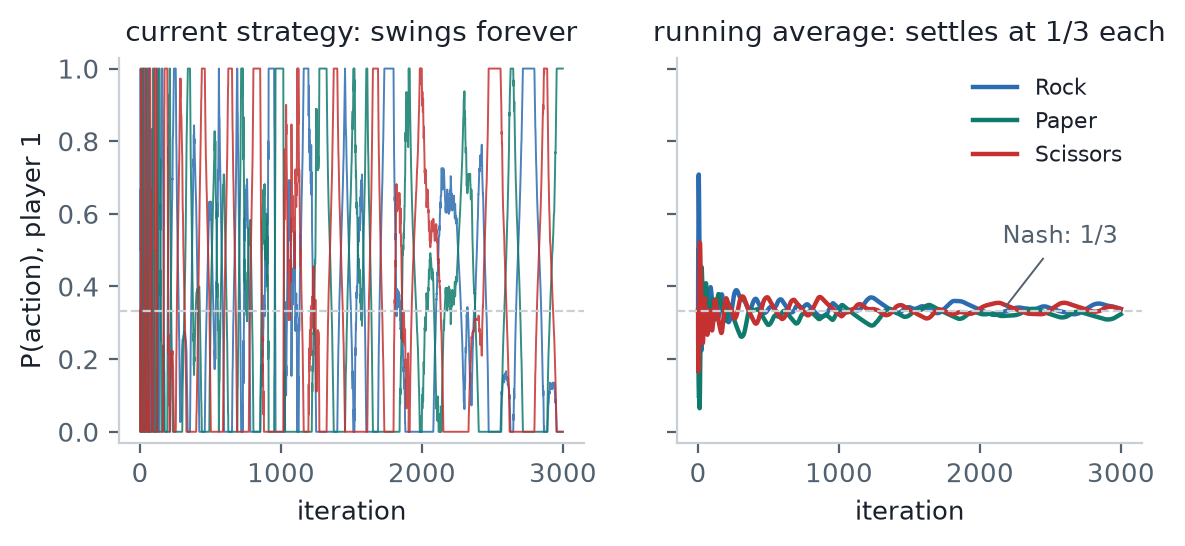
\includegraphics[width=\linewidth]{figures/rps.png}
\caption{Both players running regret matching in rock--paper--scissors (simulated for this paper): current strategy vs.\ its running average.}
\label{fig:rps}
\end{figure}

\pitfall{The single most common conceptual bug in this field is deploying or measuring the current strategy when every guarantee is about the average.} It will reappear in CFR (query the average policy), in Deep CFR (the entire reason an average-policy network exists), and in the RL section (methods that fix cycling by construction so the last iterate \emph{does} converge). Keep the distinction sharp now and the rest of the survey reads easily.
